\section{二阶线性微分方程的幂级数解法}

\subsection{方程常点邻域内的解}
蓝:由于(非常清楚地)普通的线性方程的基本解组毫无规律可言,因此用级数去近似解也是一种不错的思路。

朱鹭子:照你这么说也是确实……但用级数解法不就得考虑敛散性的问题了么?

蓝:的确,在这里我们只讨论最能接受的二阶线性微分方程:
\[
	\ddw+p(z)\dw+q(z)w=0
	.\]

并且我们给定了在 \(z_0\) 点处的初值条件,那么我们要考虑的其实是在 \(\left\vert z-z_0 \right\vert <R\) 这个圆盘上面的解,事实上:

\begin{tho}{常点附近级数解的存在性}{}
	如果 \(p(z)\) 和 \(q(z)\) 在 \(\left\vert z-z_0 \right\vert <R\)内单值解析,则方程
	\[
		\ddw+p(z)\dw+q(z)w=0
		.\]
	必然存在一个唯一解,且该唯一解在 \(\left\vert z-z_0 \right\vert <R\) 上亦单值解析。
\end{tho}
朱鹭子:解析的话就意味着条件太强了啊……

蓝:事实上这其实代表着 \(p(z)\) 在 \(q(z)\) 在 \(z_0\) 解析的情形,此时这个点被称为方程的\textbf{常点}。

朱鹭子:诶?你的意思是说即使那俩函数在 \(z_0\) 点不解析也是依然可以有解的吗?

蓝:是的,这个我们之后再讨论。由于解 \(w(z)\) 是解析的,那么我们也就可以在 \(\left\vert z-z_0 \right\vert <R\) 上将其展开成\textbf{Taylor级数}:
\[
	w(z)= \sum_{n=0}^{\infty} a_n(z-z_0)^n
	.\]

朱鹭子:看起来我只要把这方程里面的 \(p(z)\) 和 \(q(z)\) 也展开成Taylor级数,代进去就可以得到解的各个系数之间的递推公式。

蓝:看上去的确如此,但不要忘记,这个方程是有两个线性无关解的,因此你得到的递推公式可能会相当乱。

朱鹭子:这倒是。

蓝:我这里倒是有个非常不错的例子:


\begin{tcolorbox}[colback=gray!20,colframe=gray!150,fonttitle=\bfseries,arc=0mm,leftrule=1mm,toprule=0mm,bottomrule=0mm,rightrule=0mm]
	求Airy方程
	\[
		\ddw -zw=0 \tag{Airy}
		.\]
	在 \( \mathring{U}_{\varepsilon }(0)\) 上的解。
	\tcbline

	事实上容易知道这个 \(p(z)\equiv 0\) 和 \(q(z) =z\)在复平面上解析,因此不妨设解 \(w=\sum_{n=0}^{\infty} a_n z^n\),因此代入方程 (Airy) 可以用得到:
	\[
		\sum_{n=2}^{\infty} a_n n(n-1) z^{n-2}-\sum_{n=0}^{\infty} a_n z^{n+1}=0
		.\]
	整理一下就可以得到:
	\[
		2a_2+\sum_{n=1}^{\infty} ( (n+1)(n+2)a_{n+2}-a_{n-1})z^{n}=0
		.\]
	因此由Taylor展开的唯一性可以得到:
	\[
		\begin{cases}
			\\[-2.2em]
			a_2=0, \\
			(n+1)(n+2)a_{n+2}-a_{n-1}=0.
		\end{cases}
	\]
	因此我们得到了递推公式:
	\[
		\begin{cases}
			\\[-2.2em]\
			a_{3n-1}=0,                         \\
			a_{3n}= \dfrac{a_{3n-3}}{3n(3n-1)}, \\
			a_{3n+1}= \dfrac{a_{3n-2}}{3n(3n+1)},
		\end{cases}\, n\in\symbb{N} ^+.
	\]
	因此我们要考量的其实是 \(a_0\) 和 \(a_1\),实际上这两个系数就对应了方程 (Airy) 的两个线性无关解:
	\[
		a_{3n}= \frac{a_0}{\prod_{i=1}^{n} 3i(3i-1) } = \frac{a_0\prod_{i=1}^{n} (3i-2)}{(3n)!}
		.\]
\end{tcolorbox}

在这里我们不得不借助Γ函数——这个你是知道的吧?


朱鹭子:那是自然。


蓝:那就好,因此:


\begin{tcolorbox}[colback=gray!20,colframe=gray!150,fonttitle=\bfseries,arc=0mm,leftrule=1mm,toprule=0mm,bottomrule=0mm,rightrule=0mm,breakable]
	\[
		a_{3n}=\frac{a_0\prod_{i=1}^{n} (3i-2)}{(3n)!} = \frac{a_0 3^n\prod_{i=1}^{n} \left( i-\frac{2}{3} \right) }{\Gamma (3n+1)}=
		\frac{a_0 3^n \Gamma \left( n+\frac{1}{3} \right)  }{\Gamma (3n+1)\Gamma \left( \frac{1}{3} \right) }
		.\]

	用同样的手法得到:
	\[
		a_{3n+1}=	\frac{a_1 3^n \Gamma \left( n+\frac{2}{3} \right)  }{\Gamma (3n+1)\Gamma \left( \frac{1}{3} \right) }
		.\]

	因此我们就可以得到两个线性无关解:
	\[
		\begin{cases}
			\\[-2.2em]
			w_1(z)= \sum_{n=0}^{\infty} 	\dfrac{3^n \Gamma \left( n+\frac{1}{3} \right)  }{\Gamma (3n+1)\Gamma \left( \frac{1}{3} \right) } z^{3n}, \\[6pt]
			w_2(z)=\sum_{n=0}^{\infty}  \dfrac{3^n \Gamma \left( n+\frac{2}{3} \right)  }{\Gamma (3n+1)\Gamma \left( \frac{1}{3} \right) } z^{3n+1}.
		\end{cases}
	\]

	另外地,我们会设 \(\Ai(z)\coloneq\dfrac{w_1(z)}{3^{\frac{2}{3}} \Gamma \left(\frac{2}{3}\right)}-\dfrac{w_2(z)}{3^{\frac{1}{3}} \Gamma \left(\frac{1}{3}\right)},\,\Bi(z)\coloneq \dfrac{w_1(z)}{3^{\frac{1}{6}}\Gamma \left( \frac{2}{3} \right) }+\dfrac{w_2(z)}{3^{\frac{1}{6}}\Gamma \left( \frac{1}{3} \right) }\)。
\end{tcolorbox}

朱鹭子:诶?为什么要这么设呢?

蓝:事实上是这样的:

\begin{center}
	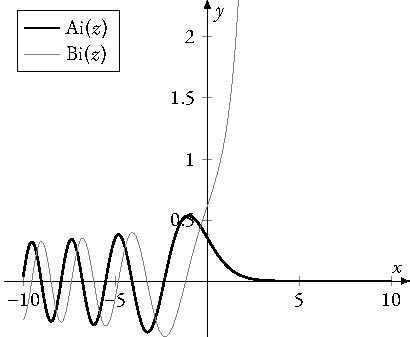
\includegraphics[]{Ai and Bi func.pdf}
\end{center}

这是两个函数的图像,\(\Ai(z)\) 在 \(z\to +\infty \) 的时候会趋向于0,实际上:
\[
	\Ai(z)\sim \frac{1}{2 \sqrt{\symup\pi }}\cdot \frac{\symrm{e} ^{-{2 z^{3/2}}/{3}}}{ \sqrt[4]{z}},\, z\to +\infty
	.\]

至于 \(\Bi(z)\) 有:
\[
	\Bi(z)\sim\frac{1}{\sqrt{\symup \pi }}\cdot  \dfrac{\symrm{e} ^{2\symrm{z} ^{3/2}/3}}{\sqrt[4]{z}},\, z\to +\infty
	.\]

我们在这里暂时先不讨论当 \(z\to \infty\) 的时候,幂级数解会变成什么样子。

好,这就是方程常点邻域内的解。同时,我们也可以根据需要进行解析延拓。
\subsection{方程极点邻域内的解}
朱鹭子:那如果不是常点呢?

蓝:不是常点那就麻烦多了,我们只讨论极点而不讨论本征奇点了。

\begin{tho}[]{极点附近级数解的存在性}{}
	如果 \(z_0\)是方程的\textbf{孤立极点},则在 \(\mathring{U}_\varepsilon (z_0)\) 上,存在两个线性无关解:\vspace{2em}
	\[
		\begin{cases}
			\\[-3.5em]
			\begin{cases}
				% \\[-2.2em]\
				\displaystyle w_1(z)=(z-z_0)^{\rho _1}\sum_{n=-\infty}^{\infty} a_n (z-z_0)^n, \\[4pt]
				\displaystyle w_2(z)=(z-z_0)^{\rho _2}\sum_{n=-\infty}^{\infty} b_n (z-z_0)^n.
			\end{cases}           & \rho _1-\rho _2\notin\symbb{Z}.           \\[30pt]
			\begin{cases}
				% \\[-2.2em]\
				\displaystyle w_1(z)=(z-z_0)^{\rho _1}\sum_{n=-\infty}^{\infty} a_n (z-z_0)^n, \\
				\displaystyle w_2(z)=gw_1(z)\ln (z-z_0)+(z-z_0)^{\rho _1}\sum_{n=-\infty}^{\infty} b_n (z-z_0)^n
			\end{cases} & \rho _1-\rho _2\in\symbb{Z}.
			\\[-1.5em]
		\end{cases}
	\]
	\vspace{0em}
\end{tho}

请允许我说明一些事情,就是这个 \(w_1(z)\ln (z-z_0) \) 的来源。

朱鹭子:请。

蓝:这段东西可能会很长,我会用一个小型盒子把它包起来。

\begin{tcolorbox}[colback=gray!20,colframe=gray!150,fonttitle=\bfseries,arc=0mm,leftrule=1mm,toprule=0mm,bottomrule=0mm,rightrule=0mm,breakable]
	\setlength{\lineskip}{5pt}
	\setlength{\lineskiplimit}{2.5pt}
	首先我们要证明的是,若 \(w_1\) 是方程:
	\[
		\symscr{D} _t^2(w)+p(z)\dw+q(t)w=0
		.\]
	的解,而且在区域 \(\symcal{I}_1\) 上解析,那么如果 \( W_1\) 是 \(w_1\) 在 \(\symcal{I} _2\) 上面的解析延拓,且 \(\symcal{I} _1 \cap\symcal{I} _2 \neq  \varnothing\),则 \( W_1\) 是方程在 \(\symcal{I} _2\) 上面的解。
	\begin{tcolorbox}[colback=gray!10,colframe=gray!40,fonttitle=\bfseries,arc=0mm,leftrule=1mm,toprule=0mm,bottomrule=0mm,rightrule=0mm,breakable]
		\color{gray!120}\kaiti
		这个的证明其实并不难,为了考虑 \( W_1\) 和 \(w_1\) 的差别,不妨构造:
		\[
			D(z)=\symscr{D} _t^2(W_1)+p(z)\symscr{D} _t(W_1)+q(t)W_1
			.\]
		我们的目的就是要证明在 \(\symcal{I} _2\) 上 \(D(z)\equiv 0\),因为 \(D(z)\) 在\(\symcal{I} _2\) 上解析,所以实际上这个函数是 \(\symscr{D} _t^2(w)+p(z)\dw+q(t)w\) 在 \(\symcal{I} _2\) 上的解析延拓,由于在 \(\symcal{I} _1 \cap\symcal{I} _2 \neq  \varnothing\) 上面 \(D(z)=D(z)=\symscr{D} _t^2(w_1)+p(z)\symscr{D} _t(w_1)+q(t)w_1\equiv 0\),故由解析延拓可知, \(D(z)\) 在\(\symcal{I} _2\) 也恒为零,因此 \(W_1(z)\) 也是方程的解。
	\end{tcolorbox}
	接下来是证明两个线性无关解 \(w_1,w_2\)的延拓\(W_1,W_2\)线性无关:
	\begin{tcolorbox}[colback=gray!10,colframe=gray!40,fonttitle=\bfseries,arc=0mm,leftrule=1mm,toprule=0mm,bottomrule=0mm,rightrule=0mm,breakable]	\color{gray!120}\kaiti
		由之前关于Wronsky行列式的讨论知道:
		\[
			\symscr{W} (t) =\symscr{W} (t_0)\exp \left( -\int_{t_0}^t p(s) \,\mathrm{d}s  \right)
			\label{wronskyhlsyupz}
			.\]
		因此考虑由\(\symcal{I}_1\)到 \(\symcal{I} _2\) 的积分路径,事实上由于 \(w_1,w_2\)线性无关,必然对于 \(\forall t_0\in\symcal{I} _1\) 都有 \(\symscr{W} (t_0)\neq 0\) ,因此沿该路线积分后,\(\symcal{I} _2\) 上的任一点也不为零,又因为\(W_1,W_2\)是方程的解,因此他们之间线性无关。
	\end{tcolorbox}
	由上面所述,由于真正的线性无关解就只有 \(w_1,w_2\) 两个,因此它们的延拓可以用其线性组合表示出来(因为其也是方程的解):
	\[
		\begin{bmatrix}
			W_1 \\    W_2 \\\end{bmatrix} =\symbfit{T}\cdot \begin{bmatrix}
			w_1 \\    w_2 \\\end{bmatrix}
		.\]
	由于 \(W_1,W_2\) 线性无关,因此 \(\left\vert\symbfit{T}  \right\vert \neq 0\)。

	现在我们考虑一种特殊的延拓,那就是 \(w_1,w_2\) 沿着 \(z_0\) 旋转一周时候的解析延拓 \(W_1,W_2\) (依然使用这个记法,后续中我们默认用大写表示解析延拓)。这样做是为了方便讨论 \(w_1,w_2\) 本身的多值性。

	考虑一种特殊的解:
	\[
		w_{\mathrm{m} }= a_1 w_1 +a_2w_2 = \begin{bmatrix}
			a_1 & a_2 \\
		\end{bmatrix}\cdot \begin{bmatrix}
			w_1 \\    w_2 \\\end{bmatrix}
		.\]
	满足:\(W_{\mathrm{m} } = \lambda w_{\mathrm{m}}\),这样做是为了方便讨论。

	事实上,这样的 \(w_{\mathrm{m}}\) 必然是存在的,因为:
	\[
		W_{\mathrm{m}} =  \begin{bmatrix}
			a_1 & a_2 \\
		\end{bmatrix}\cdot \begin{bmatrix}
			W_1 \\    W_2 \\\end{bmatrix} =  \begin{bmatrix}
			a_1 & a_2 \\
		\end{bmatrix}^{\symrm{T}}\cdot  \symbfit{T} \cdot \begin{bmatrix}
			w_1 \\    w_2 \\\end{bmatrix}= \lambda w_{\mathrm{m}} =\lambda \cdot  \begin{bmatrix}
			a_1 & a_2 \\
		\end{bmatrix}\cdot \begin{bmatrix}
			w_1 \\    w_2 \\\end{bmatrix}
		.\]
	考虑到 \(\begin{bmatrix}
		w_1 \\    w_2 \\\end{bmatrix}\) 是线性无关的,因此 \(\lambda \) 实际上是矩阵 \(\symbfit{T} \) 的特征值,由于\(\left\vert\symbfit{T}  \right\vert \neq 0\),因此必然存在(而且不为零),只是有无重根的区别罢了。
	\begin{itemize}\kaiti
		\item 现在先考虑没有重根 \(\lambda_1,\lambda _2\)的情况,此时两个线性无关解中必然有一个多值函数,因为我们按照上面的求法得到了 \(w_{\mathrm m,\lambda_1}\) 与 \(w_{\mathrm m,\lambda _2}\) 必然是线性无关的,否则必然有
		      \[
			      \dfrac{w_{\mathrm m,\lambda_1}}{w_{\mathrm m,\lambda _2}}=c_1 \implies \dfrac{W_{\mathrm m,\lambda_1}}{W_{\mathrm m,\lambda _2}} = \dfrac{\lambda_1 }{\lambda _2}\cdot\dfrac{w_{\mathrm m,\lambda_1}}{w_{\mathrm m,\lambda _2}} = \dfrac{\lambda_1 }{\lambda _2}\cdot c_1
		      \]
		      但同时 \(\dfrac{W_{\mathrm m,\lambda_1}}{W_{\mathrm m,\lambda _2}} \) 也是解析的,事实上它是 \(c_1\) 的解析延拓,因此必然有 \(\dfrac{W_{\mathrm m,\lambda_1}}{W_{\mathrm m,\lambda _2}}\equiv c_1\),这就得到了 \( \dfrac{\lambda_1}{\lambda _2}=1\) 与两根相异矛盾。

		      因此我们将会得到两个线性无关的 \(W_{\mathrm{m}}\) ,而观察到绕一圈之后其值会有变化(如果没有变化要求 \(\lambda =1\) ,但因为此时讨论 \(\lambda \)有两个不同根的情况,故必然要讨论多值函数)。这意味着我们即使连在 \(z_0 \) 附近将解展开成Laurent级数都做不到。

		      但另外一件事是这个函数:
		      \[
			      g(z)\coloneq (z-z_0)^{ \frac{\ln \lambda }{2\symup \pi\symrm{i} }}
			      .\]
		      当然正常情况下是多值的,其绕 \(z_0\)一圈后的延拓 \(G(z) = \exp\left( 2\symup \pi \symrm{i} \cdot  \dfrac{\ln \lambda }{2\symup \pi\symrm{i} }\right)\cdot (z-z_0)^{ \frac{\ln \lambda }{2\symup \pi\symrm{i} }}=\lambda g(z)\),这意味着如果 \(w_{\mathrm{m}}\) 和 \(g(z)\) 同时绕 \(z_0\) 一圈进行延拓,那么他们的商会互相抵消,也就是:
		      \[
			      \dfrac{w_{\mathrm{m}}}{g(z)}\, \mbox{\kaiti 是单值的}
			      .\]
		      又由于解析性,因此我们可以认为 \(\dfrac{w_{\mathrm{m}}}{g(z)}\)在整个延拓域(包括原域)都是\textbf{单值解析}的,那么就可以将其展开成Laurent级数:
		      \[
			      \dfrac{w_{\mathrm{m}}}{g(z)}=\sum_{n=-\infty}^{\infty} a_n (z-z_0)^n \implies w_{\mathrm{m}} = (z-z_0)^{ \frac{\ln \lambda }{2\symup \pi\symrm{i} }} \sum_{n=-\infty}^{\infty} a_n (z-z_0)^n
			      .\]
		      由于这样的 \(w_{\mathrm{m}}\) 有两个,不妨设 \( \rho =  \dfrac{\ln \lambda }{2\symup \pi\symrm{i} }\) ,则就得到了我们定理的第一部分:
		      \[
			      \begin{cases}
				      \displaystyle w_1(z)=(z-z_0)^{\rho _1}\sum_{n=-\infty}^{\infty} a_n (z-z_0)^n, \\[4pt]
				      \displaystyle w_2(z)=(z-z_0)^{\rho _2}\sum_{n=-\infty}^{\infty} b_n (z-z_0)^n.
			      \end{cases}  \, \rho _1-\rho _2\notin\symbb{Z}.
		      \]
		      这里的 \(\rho _1-\rho _2\notin\symbb{Z}\) 是为了让 \( \exp (2\symup \pi \symrm{i} \rho_1 )\neq\exp (2\symup \pi \symrm{i} \rho_2 )\) ,即 \(\lambda_1\neq \lambda _2\)。
		\item 现在来考虑如果矩阵 \(\symbfit{T} \) 的特征值有重根的情形:此时我们只能找到一个 \(w_{\mathrm{m},\lambda_1}\) ,为了找到另外的解 \(w_{\rm a}\)(且与 \(w_{\mathrm{m},\lambda_1 }\) 线性无关),我们考虑:
		      \[
			      W_{\rm a} = \begin{bmatrix}
				      b_1 & b_2 \\\end{bmatrix}^{\symrm{T} } \cdot \begin{bmatrix}
				      w_{\mathrm{m},\lambda_1} \\    w_{\rm a} \\\end{bmatrix}
			      .\]
		      此时实际上是用 \(w_{\mathrm{m},\lambda_1}\) 和 \(w_{\rm a}\) 两个函数作为基来表示微分方程的解空间,
		      \[
			      \begin{bmatrix}
				      W_{\mathrm m,\lambda_1 } \\  W_{\rm a}   \\\end{bmatrix}=\symbfit{T}_{\rm new} \cdot   \begin{bmatrix}
				      w_{\mathrm{m},\lambda_1} \\    w_{\rm a} \\\end{bmatrix}=\begin{bmatrix}
				      \lambda_1 & b_1 \\
				      0         & b_2 \\
			      \end{bmatrix}\cdot \begin{bmatrix}
				      w_{\mathrm{m},\lambda_1 } \\    w_{\rm a} \\\end{bmatrix}
			      .\]
		      考虑到我们为了找到 \(w_{\mathrm{m}}\) 在这个矩阵下面的表示,我们要求它的特征值,但是 \( w_{\mathrm{m}}\) 对应的特征值是不会矩阵 \(\symbfit{T} \) 和 \( \symbfit T_{\rm new}\)  所影响,因此 \( \symbfit T_{\rm new}\) 的特征值依然是 \( \lambda_1\) 这样实际上就是:
		      \[
			      \left\vert \symbfit T_{\rm new}- \lambda \symbfit E \right\vert = 0 \implies(\lambda_1-\lambda )(b_2-\lambda )=0
			      .\]
		      我们清楚知道 \(\lambda_1\) 是二重根,因此 \(b_2=\lambda_1\)。这就意味着:
		      \[
			      W_{\rm a}=a_1 w_{\mathrm{m},\lambda_1}+ w_{\rm a}
			      .\]
		      以及
		      \[
			      W_{\mathrm{m},\lambda_1}= \lambda_1w_{\mathrm{m},\lambda_1}
			      .\]
		      得到:
		      \[
			      \frac{W_{\rm a}}{W_{\mathrm{m},\lambda_1}}= \frac{w_{\rm a}}{w_{\mathrm{m},\lambda_1}}+ \frac{b_1}{\lambda_1}
			      .\]
		      这就意味着函数 \(\dfrac{w_{\rm a}}{w_{\mathrm{m},\lambda_1}}\) 绕 \(z_0\) 点一周之后,它的值会增加 \( \dfrac{b_1}{\lambda_1}\),实际上 \( \dfrac{b_1}{\lambda_1} \cdot \dfrac{\ln (z-z_0)}{2\symup \pi \symrm{i} }\) 也是如此,因此:
		      \[
			      \frac{w_{\rm a}}{w_{\mathrm{m},\lambda_1}}-\dfrac{b_1}{\lambda_1} \cdot \dfrac{\ln (z-z_0)}{2\symup \pi \symrm{i} }\,\mbox{\kaiti 是单值的}
			      .\]
		      然后把它展开成Laurent级数:

	\end{itemize}
	\[
		\frac{w_{\rm a}}{w_{\mathrm{m},\lambda_1}}-\dfrac{b_1}{\lambda_1} \cdot \frac{\ln (z-z_0)}{2\symup \pi \symrm{i} }=\sum_{n=-\infty}^{\infty} c_n (z-z_0)^n\implies w_{\rm a} =gw_{\mathrm{m},\lambda_1}\ln (z-z_0)+(z-z_0)^{\rho _1}\sum_{n=-\infty}^{\infty} d_n (z-z_0)^n
		.\]
\end{tcolorbox}
到这里就结束了。

朱鹭子:好!酣畅淋漓!但是我有一些问题,首先,我们是要知道具体的 \(\rho _1\) 和 \(\rho _2\) 长什么样子才能知道这个解的形式到底有无对数,而要求 \(\rho _1\)和 \(\rho _2\) 就必须要求得解的形式,这是否算一种循环?另外一件事情是,经过上面的讨论,其实和 \(p(z),q(z)\) 在 \(z_0\) 点的解析性无关,为何当他们都是解析函数的时候,微分方程的解没有对数项?

蓝:好问题,事实上 \(\rho _1\) 与 \(\rho _2\) 我们有办法在不求出解的形式而进行讨论,这点后面在说明,至于为什么解析的方程的解也是解析的,此处我做一些简短的说明。

事实上,这个二阶微分方程其实等价求解:
\[
	\ddw= - p(z)\dw-q(z)w
	.\]
不妨设 \(u=\dw\) ,则不妨认为 \(u\) 是下面问题的解:
\[
	\symscr{D} _z(u) = -p(z) u - q(z) w
	.\]

此时看起来像个正常的一阶方程,但实际上 \(w\) 的存在性不明,因此我们依然要想办法找个函数序列趋近 \(w\),事实上我们完全可以:
\[
	\begin{cases}
		\symscr{D} _z(u) = -p(z) u - q(z) v , \\
		\symscr{D} _z(v) = -\dfrac{\symscr{D} _z(u)}{p(z)}- \dfrac{q(z)}{p(z)} v.
	\end{cases}
\]

事实上 \(u\) 和 \(v\) 分别对应了解 \(\dw\) 和 \(w\)(如果存在的话),因此在有初值条件:
\[
	w(z_0)=w_0,\,w'(z_0)=w_0'
	.\]

因此我们就可以按照以下方法进行迭代:
\[
	\begin{aligned}
		 & u_0 = w_0' ,                                                                                               \\
		 & v_0=w_0    ,                                                                                               \\
		 & u_{n+1}(z) = w_0'-\int_{z_0}^z \left( p(s) u_n(s) + q(s) v_n(s) \right) \,\mathrm{d}s              ,       \\
		 & v_{n+1}(z) = w_0-\int_{z_0}^z \left( \dfrac{u_n(s) }{p(z)}+\dfrac{q(z)}{p(z)}v_n(s) \right) \,\mathrm{d}s.
	\end{aligned}
\]

然后再证明 \(u_i\) 和 \(v_i\) 都存在极限 \(u_{\rm m}\) 和 \(v_{\rm m}\),此就代表了二阶线性方程满足初值条件的解,具体证法可以参照一阶微分方程存在性定理的Picard证法(当然此处还要证明解析,但实际上只要求证明某些序列比如 \(u_{n+1}-u_{n}\)一致收敛即可),此处不再赘述。

朱鹭子:那也算行,现在的问题是,你这个定理,它得到的那个 Laurent 级数的幂是从负无穷到正无穷,这样做是否会……

蓝:是,会非常麻烦,比如看看:
\[
	\sum_{n=-\infty}^{\infty} \frac{a_{n+2}(z-z_0)^n}{(\rho _1+n)(\rho _1+n-1)} +\underline{\sum_{n=-\infty}^{\infty} \sum_{j=-k}^{\infty}}\frac{a_{n+1}b_j(z-z_0)^{n+j}}{\rho _1+n}  +\underline{\sum_{n=-\infty}^{\infty} \sum_{j=-m}^{\infty}} a_n c_j (z-z_0)^{n+j}=0
	.\]

下划线部分的两个求和并没有什么好的处理方法,因为有一个从负无穷到正无穷的积分,你没有办法利用Cauthy乘积化简:
\[
	\sum_{n=0}^{\infty} a_k \cdot \sum_{n=0}^{\infty} b_k = \sum_{n=0}^{\infty} \left( \sum_{i=0}^{n} a_i b_{n-i} \right)
	.\]

在这里做是没有意义的,因为你依然会得到一个含有无穷求和的方程才能确定 \(z^i\) 的系数。

朱鹭子:原来如此,那怎么样才能化简这个呢?

蓝:暂时没有什么好的方法。

朱鹭子:\emoji{😂}。啊这……

蓝:但有另外一种类型的方程,这种方程的解是正常的:
\vspace{1em}
\[
	\begin{cases}
		% \\[-2.2em]\
		\displaystyle w_1(z)=(z-z_0)^{\rho _1}\sum_{n=0}^{\infty} a_n (z-z_0)^n, \\
		\displaystyle w_2(z)=gw_1(z)\ln (z-z_0)+(z-z_0)^{\rho _2}\sum_{n=0}^{\infty} b_n (z-z_0)^n,
	\end{cases}\quad  \rho _1-\rho _2\in\symbb{Z}.
\]
\vspace{0em}

注意到这些解并不是从负无穷开始求和的,因此我们有希望求出它们的解,此时的解被称为\textbf{正则的}。正则的就是好的。

朱鹭子:正则的就是好的。

蓝:\emoji{✔}

蓝:当然此时 \(z_0\) 依然是方程的奇点,但是由于可以诱导正则解,所以是\textbf{正则奇点}。

朱鹭子:正则的就是好的。

蓝:\emoji{✔}

朱鹭子:那正则奇点有满足上面条件呢,就那个微分方程?

蓝:事实上这个方程是有充要条件的:
\begin{tho}{二阶线性微分方程有两个线性无关正则解的充要条件}{}
	对于方程
	\[
		\ddw+p(z)\dw+q(z)w=0
		.\]
	在 \(z_0\) 邻域内有两个线性无关的正则解的充要条件是 \((z-z_0)p(z)\) 和 \((z-z_0)^2 q(z)\) 在 \(z_0\) 点解析。
\end{tho}


由\hyperref[wronskyhlsyupz]{\underline{这里的讨论}}我们知道:
\[
	\begin{aligned}
		\symscr{W} (z) & =\symscr{W} (z_0)\exp \left( -\int_{z_0}^z p(s) \,\mathrm{d}s  \right) \implies p(z) =-\symscr{D} _z\left( \ln \left( \frac{\symscr{W} (z)}{\symscr{W} (z_0)} \right)  \right)    \\
		               & =-\symscr{D} _z (\ln (w_1\symscr{D} _z(w_2)-w_2\symscr{D} _z(w_1))) = -\symscr{D} _z\left( \ln \left( w_1^2\cdot \symscr{D} _z\left(  \frac{w_2}{w_1} \right)  \right)  \right) .\end{aligned}
\]

然后可以尝试下一股脑代进去,就用上面正则解的形式:


\[
	\begin{aligned}
		p(z) & =-\symscr{D} _z\left( \ln \left( w_1^2\cdot \symscr{D} _z\left(  \frac{w_2}{w_1} \right)  \right)  \right)                                                                                                                                   \\
		     & =-\symscr{D} _z\left( \ln \left( w_1^2\cdot \symscr{D} _z\left(  \frac{gw_1(z)\ln (z-z_0)+(z-z_0)^{\rho _2}\sum_{n=0}^{\infty} b_n (z-z_0)^n}{(z-z_0)^{\rho _1}\sum_{n=0}^{\infty} a_n (z-z_0)^n} \right)  \right)  \right)                  \\
		     & =-\symscr{D} _z\left( \ln \left( w_1^2\cdot \symscr{D} _z\left( g \ln (z-z_0)+ (z-z_0)^{\rho _2-\rho _1}\frac{\sum_{n=0}^{\infty} b_n (z-z_0)^n}{\sum_{n=0}^{\infty} a_n (z-z_0)^n} \right)  \right)  \right)                                \\
		     & =-\symscr{D} _z\left( \ln \left( w_1^2\cdot \symscr{D} _z\left( g \ln (z-z_0)+ (z-z_0)^{\rho _2-\rho _1} \sum_{n=0}^{\infty} k_n (z-z_0)^n \right)  \right)  \right)                                                                         \\
		     & =-\symscr{D} _z\left( \ln \left( w_1^2\cdot \left( \frac{g}{z-z_0}+ (z-z_0)^{\rho _2-\rho _1} \sum_{n=0}^{\infty} (\rho _2-\rho _1+n)k_n (z-z_0)^n \right)  \right)  \right)                                                                 \\
		     & =-\symscr{D} _z\left( \ln \left( (z-z_0)^{2\rho _1}\left( \sum_{n=0}^{\infty} a_n (z-z_0)^n \right)^2 \cdot \left( \frac{g}{z-z_0}+ (z-z_0)^{\rho _2-\rho _1} \sum_{n=0}^{\infty} (\rho _2-\rho _1+n)k_n (z-z_0)^n \right)  \right)  \right) \\
		     & =-\symscr{D} _z\left( \ln \left( \sum_{n=-1}^{\infty} A_n (z-z_0)^{n+2\rho _1}  + (z-z_0)^{\rho _2+\rho _1} \sum_{n=0}^{\infty}B_n(z-z_0)^n \right)  \right)                                                                                 \\
		     & =- \frac{\sum_{n=-1}^{\infty} C_n (z-z_0)^{n+2\rho _1-1}  + (z-z_0)^{\rho _2+\rho _1} \sum_{n=0}^{\infty}D_n(z-z_0)^{n-1}}{\sum_{n=-1}^{\infty} A_n (z-z_0)^{n+2\rho _1}  + (z-z_0)^{\rho _2+\rho _1} \sum_{n=0}^{\infty}B_n(z-z_0)^n}
	\end{aligned}
	.\]

因此:
\[
	zp(z)=- \frac{\sum_{n=-1}^{\infty} C_n (z-z_0)^{n+2\rho _1}  + (z-z_0)^{\rho _2+\rho _1} \sum_{n=0}^{\infty}D_n(z-z_0)^{n}}{\sum_{n=-1}^{\infty} A_n (z-z_0)^{n+2\rho _1}  + (z-z_0)^{\rho _2+\rho _1} \sum_{n=0}^{\infty}B_n(z-z_0)^n}
	.\]

在 \(z_0\) 是可去奇点,又因为分母分子解析,所以这玩意实际上就是在 \(z_0\) 邻域内解析,故 \(zp(z)\) 在 \(z_0\) 邻域内解析。至于 \(q(z)\)……

实际上:
\[
	q(z)=- \frac{\symscr{D} _z^2(w_1)}{w_1}-p(z) \frac{\symscr{D} _z(w_1)}{w_1}
	.\]

且由于上面的讨论得到 \(z_0\) 是 \(p(z)\) 的最多一阶极点,因此可以得到 \(z_0\) 是 \(q(z)\) 的最多二阶极点。因此就完成了必要性的证明。

朱鹭子:别写了,没人会看计算过程的,提及一下即可。

蓝:好,接下来是充分性由于时间问题暂且不论了,接下来我们要讨论的是如何求出 \(\rho _1\) 和 \(\rho _2\) ,这被称为方程在正则奇点处的\textbf{指标}。为了方便讨论,以后不妨设 \(\Re(\rho _1)\geqslant \Re(\rho _2)\)。

由于解的形状是就是那两种,而那个 \(\ln (z-z_0)\) 是不会影响 \((z-z_0)\) 的幂的,因为不能展开,因此我们不妨设解的形式为:
\[
	w(z) = (z-z_0)^{\rho } \sum_{n=0}^{\infty} w_n(z-z_0)^n
	.\]

同时我们也将 \(p(z)\) 和 \(q(z)\) 展开:
\[
	p(z)=\sum_{n=0}^{\infty} p_n (z-z_0)^{n-1},\,q(z)= \sum_{n=0}^{\infty} q_n (z-z_0)^{n-2}
	.\]

一股脑代进去就可以得到:
\[
	\begin{aligned}
		    & (z-z_0)^{\rho } \sum_{n=0}^{\infty}(n+\rho )(n+\rho -1) w_n(z-z_0)^{n-2}                            \\
		+\, & (z-z_0)^{\rho } \sum_{i=0}^{\infty} p_i (z-z_0)^{i-1}\sum_{n=0}^{\infty}(n+\rho ) w_n (z-z_0)^{n-1} \\
		+\, & (z-z_0)^{\rho }\sum_{i=0}^{\infty} q_i (z-z_0)^{i-2} \sum_{n=0}^{\infty} w_n(z-z_0)^n =0.
	\end{aligned}
\]

观察到 \((z-z_0)^{\rho -2}\) 是可以约掉的,则:
\[
	\begin{aligned}
		    & \sum_{n=0}^{\infty}(n+\rho )(n+\rho -1) w_n(z-z_0)^{n}:                          & M_1 \\
		+\, & \sum_{i=0}^{\infty} p_i (z-z_0)^{i}\sum_{n=0}^{\infty}(n+\rho ) w_n (z-z_0)^{n}: & M_2 \\
		+\, & \sum_{i=0}^{\infty} q_i (z-z_0)^{i} \sum_{n=0}^{\infty} w_n(z-z_0)^n:            & M_3
	\end{aligned}
\]

由于东西比较多,不妨分而治之,首先考虑 \(M_2\):
\[
	\sum_{i=0}^{\infty} p_i (z-z_0)^{i}\sum_{n=0}^{\infty}(n+\rho ) w_n (z-z_0)^{n}= \sum_{n=0}^{\infty}\sum_{i=0}^{\infty} w_n p_i (n+\rho ) (z-z_0)^{n+i}\xlongequal[]{\mbox{\tiny Cauthy乘积}}\sum_{n=0}^{\infty}\sum_{i=0}^{n} w_{i} p_{n-i} (i+\rho ) (z-z_0)^{n}
	.\]


然后是 \(M_3\) :
\[
	\sum_{n=0}^{\infty}\sum_{i=0}^{\infty} q_i  w_n(z-z_0)^{n+i}\xlongequal[]{\mbox{\tiny Cauthy乘积}}\sum_{n=0}^{\infty}\sum_{i=0}^{n} q_{n-i} w_i (z-z_0)^n
	.\]

因此实际上就有(上面三者加起来):
\[
	\label{CON}
	\sum_{n=0}^{\infty}\left( (n+\rho )(n+\rho -1)w_n+\sum_{i=0}^{n}( p_{n-i} (i+\rho ) + q_{n-i})w_{i} \right) z^n=0 \tag{CON}
	.\]

朱鹭子:看起来倒终于像个正经的级数了。

蓝:的确,为了求出 \(\rho \) ,我们把 \(n=0\) 这一项拿出来:
\[
	\rho (\rho -1)w_n +(\rho  p_0+q_0)w_0=0\implies \underline{\rho ^2+(p_0-1)\rho +q_0=0}
	.\]

此时我们完全可以令 \(w_0\neq 0\),因为如果 \(w_0=0\),此时可以通过调整 \(\rho \) 让新 \(w_0\neq 0\)。

上式就是指标要满足的方程,被称为\textbf{指标方程}。根据这个方程我们就可以求得 \(\rho _1\)和 \(\rho _2\)。接下来我们需要借助 \(\rho _1\) 和 \(\rho _2\) 的情况去讨论对数项的形式。

\begin{itemize}\kaiti
	\item \(\rho _1=\rho _2\),此时根据上面的讨论,对应的是矩阵 \(\symbfit{T} \)的特征值有重根的情形,而且此时的情况是,由于递推是线性的,我们两个 \(\rho _1\) 与 \(\rho _2\) 代进去得到的解必然是线性相关的,因此不含对数项是不行的。
	\item 如果 \(\rho _1-\rho _2\notin\symbb{Z} \) ,这实际上意味着我们把  \(\rho _1\) 与 \(\rho _2\) 代进去得到的解的\textbf{幂}完全不同,必然是线性无关的,此时该两个解就是微分方程的线性无关解,对数项也没有存在的必要了。
	\item \(\rho _1-\rho _2\in\symbb{Z}/\{0\} \),此时是相当特殊的情况,如果\(\rho _1-\rho _2\notin\symbb{Z}/\{0\} \),那么我们 \(w_n\) 的通项可以这么表示:
	      \[
		      w_n= -\dfrac{\sum_{i=0}^{n-1}( p_{n-i} (i+\rho ) + q_{n-i})w_{i}}{ (n+\rho )(n+\rho -1)+p_0(n+\rho )+q_0}\propto w_0
		      .\]

	      注意看!如果 \(\rho _1-\rho _2\) 是非零整数 \(m\)的话(由于前面规定说 \(\Re(\rho _1)\geqslant \Re(\rho _2)\),因此 \(m\geqslant 1\)),这意味着,我们求完 \(\rho _1\) 对应的解(这里并不会有什么问题)之后求 \(\rho _2\) 对应的解是,会碰到:
	      \[
		      \begin{aligned}
			      w_m & = -\dfrac{\sum_{i=0}^{m-1}( p_{m-i} (i+\rho _2 ) + q_{m-i})w_{i}}{ (m+\rho _2 )(m+\rho _2 -1)+p_0(m+\rho _2 )+q_0} \\
			          & \implies (\rho _1(\rho _1 -1)+p_0\rho _1 +q_0)w_m+{\sum_{i=0}^{m-1}( p_{m-i} (i+\rho _2 ) + q_{m-i})w_{i}}=0.
		      \end{aligned}
	      \]

	      其中 \(w_m\) 的系数是指标方程,故为零,因此如果 \(\sum_{i=0}^{m-1}( p_{m-i} (i+\rho _2 ) + q_{m-i})w_{i}\neq 0\),此时这样的形式必然没有解,换句话说,我们只能求出一种 \(\displaystyle (z-z_0)^{\rho _1}\sum_{n=0}^{\infty} a_n (z-z_0)^n\) 形式的解,因此对数项就有了存在的必要。如果 \(\sum_{i=0}^{m-1}( p_{m-i} (i+\rho _2 ) + q_{m-i})w_{i}=0\),此时 \(w_m\) 的值无关紧要,完全可以认为是零(事实上不认为是零也一样的,只不过从 \(w_m\)往后的部分实际上将会是第一个解的一部分)。
\end{itemize}

朱鹭子:好!这就是全部的讨论?

蓝:差不多了,接下来我们来看个例子,由于例子比较长,我要用一个 subsection 来包裹它。

\subsection{Bessel方程}

蓝:Bessel方程的形状是:
\[
	\ddw+\frac{\dw}{z}+ \left( 1- \frac{\nu^2}{z^2 } \right) w=0,\, \Re(\nu )\geqslant 0
	.\]

这玩意来源于Helmholtz方程:
\[
	\nabla^2u+k^2 u=0
	.\]
在柱坐标系下的分离变量,此处不管。现在我们观察这个方程,首先 \(z=0\) 是方程的正则奇点,\(z=\infty\) 不讨论。在这里主要讨论方程在 \(z=0\) 的空心邻域 \(\left\vert z \right\vert >0\) 上的解。
设:
\[
	w(z)=z^\rho \sum_{n=0}^{\infty} w_n z^{n}
	.\]
代入方程 \hyperref[CON]{\underline{(CON)}}就可得到指标方程:
\[
	\rho ^2-\nu ^2=0 \implies \rho _1=\nu ,\,\rho _2=\nu \implies rho_1-\rho _2=2\nu
	.\]
和正儿八经的递推关系:
\[
	w_n((\rho +n)^2-\nu ^2)+w_{n-2}=0,\,n\geqslant 2
	.\]

因此承担分离出两个线性无关解的任务(看似)就落到了 \(w_0\) 和  \(w_1\) 头上。我们按部就班讨论。

\begin{itemize}\kaiti
	\item \(2\nu \in\symbb{Z} \) 时,此时并没有对数什么关系,因此按部就班:
	      \[
		      w_n= -\frac{w_{n-2}}{(\rho +n)^2-\nu ^2}=-\frac{w_{n-2}}{n(n+2\rho )}
		      .\]
	      因此:
	      \[
		      \begin{aligned}
			      w_{2n}   & = -\frac{w_{2n-2}}{2n(2n+2\rho )}=\frac{w_{2n-4}}{2n(2n+2\rho )(2n-2)(2n-2+2\rho )}                                                                                                         \\
			               & =\dotsm\frac{(-1)^nw_0}{\prod_{i=1}^{n} (2i)(2i+2\rho )}=\frac{(-1)^nw_0}{4^n \Gamma (n+1)\prod_{i=1}^{n}(i+\rho )}=\frac{(-1)^n \Gamma (\rho +1)w_0}{4^n \Gamma (n+1) \Gamma (\rho +n+1)}. \\
			      w_{2n+1} & = -\frac{w_{2n-1}}{(2n+1)(2n+1+2\rho )} =\cdots \frac{(-1)^nw_1}{\prod_{i=1}^{n} (2i+1)(2i+1+2\rho )}                                                                                       \\
			               & = \frac{(-1)^nw_1}{4^n\prod_{i=1}^{n}\left( i+\frac{1}{2} \right) \left( i+\rho +\frac{1}{2} \right) }=
			      \frac{(-1)^n \Gamma (\frac{3}{2})\Gamma \left( \rho +\frac{3}{2} \right) w_1}{4^n \Gamma \left( n+\frac{3}{2} 	\right) \Gamma \left( n+\rho +\frac{3}{2} \right)  }.
		      \end{aligned}
	      \]
\end{itemize}

朱鹭子:等等!你这有问题吧,由于 \(w_{2n}\) 和 \(w_{2n-1}\) 是相互独立的,那就代表了两个线性无关解,但这样不就是…… 一个 \(\rho \) 对应两个线性无关解??????那最后不是就有四个解了吗?

蓝:所以我才说出两个线性无关解的任务(\textbf{看似})就落到了 \(w_0\) 和  \(w_1\) 头上,但事实上有些东西会影响到我们对 \(w_0\) 和 \(w_1\) 的选取,而且并不是初始条件!比如这个所谓的正儿八经的递推关系实际上是不完全的,代进去事实上会得到:
\[
	\begin{aligned}
		           & \sum_{n=0}^{\infty} w_n\left( (n+\rho )^2-\nu ^2 \right) z^n +\sum_{n=0}^{\infty} w_n z^{n+2}=0                        \\
		\implies\, & c_0(\rho ^2-\nu ^2)+c_1((\rho +1)^2-\nu ^2)z+\sum_{n=2}^{\infty} \left[ w_n((\rho +n)^2-\nu ^2)+w_{n-2} \right] z^n=0.
	\end{aligned}
\]

考虑到 \(z^1\) 的系数 \(c_1((\rho +1)^2-\nu ^2)=0\) ,我们立马就可以得到……

朱鹭子:\(c_1=0\)?哦不对,由于 \(\rho =\pm\nu \) 实际上是 \(\nu \neq \dfrac{1}{2}\) 的时候 \(c_1=0\) ,那么实际上此时所有的 \(w_{2n+1}\) 就都是零了。

蓝:对,此时实际上只有正经的一个解:
\[
	w= z^\rho  \sum_{n=0}^{\infty} \frac{(-1)^n \Gamma (\rho +1)w_0}{4^n \Gamma (n+1) \Gamma (\rho +n+1)}z^{2n}=z^\nu   \sum_{n=0}^{\infty} \frac{(-1)^n \Gamma (\rho +1)w_0}{\Gamma (n+1) \Gamma (\rho +n+1)} \left( \frac{z}{2} \right) ^n
	.\]

不妨设 \(w_0=\dfrac{1}{2^\nu  \Gamma (\nu +1)}\),因此得到:
\[
	w= \sum_{n=0}^{\infty} \frac{(-1)^n}{\Gamma (n+1)\Gamma (n+\nu +1)} \left( \frac{z}{2} \right) ^{2n+\nu }\eqcolon \besselj_\nu(z)
	.\]

这被称为\textbf{第一类Bessel函数}。此时令 \(\rho =-\nu \) 的时候可以得到:
\[
	\besselj_{-\nu}(z)_ = \sum_{n=0}^{\infty} \frac{(-1)^n}{\Gamma (n+1)\Gamma (n-\nu +1)} \left( \frac{z}{2} \right) ^{2n-\nu }
	.\]

事实上你会发现虽然对应的是不同的 \(\rho \) 但两解的形式殊途同归,当然此时是在 \(2\nu \notin\symbb{Z} \) 的情况下推出来的。

朱鹭子:那如果是整数呢?

蓝:整数那就麻烦了。我们先来看看之前那个 \(\nu =\dfrac{1}{2}\) 的情况吧。此时我们知道 \(w_1\) 可以任意取值,我们取 \(0\) 的话,实际上会得到第二个解变成下面这种:
\[
	w_{\rho =-\frac{1}{2}} = \underset{\kaiti 按照之前方法求出来的部分}{\underbrace{\sum_{n=0}^{\infty} \frac{(-1)^n}{\Gamma (n+1)\Gamma \left( n-\frac{1}{2} +1 \right) } \left( \frac{z}{2} \right) ^{2n-\frac{1}{2} }}} + \underset{z^{-1 /2}\sum_{n=0}^{\infty} 	 \frac{(-1)^n \Gamma\left(3 /2\right) w_1}{4^n \Gamma \left( n+3 /3	\right) \Gamma \left( n+1 \right)  } z^{2n+1}=w_1 \Gamma \left( \frac{3}{2} \right)  \cdot \besselj_{1/2}(z)
	}{\underbrace{z^{-\frac{1}{2}}\sum_{n=0}^{\infty} 	 \frac{(-1)^n \Gamma (\frac{3}{2})\Gamma \left( \rho +\frac{3}{2} \right) w_1}{4^n \Gamma \left( n+\frac{3}{2} 	\right) \Gamma \left( n+\rho +\frac{3}{2} \right)  } z^{2n+1}}} = \besselj_{-\frac{1}{2}}(z) +w_1\sqrt{ \frac{\symup\pi }{2}}\besselj_{\frac{1}{2}}(z)
	.\]

发现得到的结果殊途同归,只是加上了第一个解乘上一个常数罢了。

接下来我们看看其他 \(\nu \in \symbb{Z} +\dfrac{1}{2}\) 的情况,此时这微分方程的解是有初等表达的。

朱鹭子:我超!!原来是有初等表达的。

蓝:是。我们知道此时我们先尝试代入 \(\mathrm J_ \nu (z)\) 和 \( \mathrm J_ {-\nu }(z)\),看他们是否线性相关吧。

\[
	\begin{aligned}
		\mathrm J_ {k+\frac{1}{2}} (z) = \sum_{n=0}^{\infty} \frac{(-1)^n}{\Gamma (n+1)\Gamma (n+k +3 /2)} \left( \frac{z}{2} \right) ^{2n+k +\frac{1}{2} } \\
		\mathrm J_ {-k-\frac{1}{2}} (z) = \sum_{n=0}^{\infty} \frac{(-1)^n}{\Gamma (n+1)\Gamma (n-k -3 /2)} \left( \frac{z}{2} \right) ^{2n-k -\frac{1}{2} }
	\end{aligned}
	.\]

朱鹭子:最低次幂都不一样,怎么可能线性相关?

蓝:(笑)也是,接下来我们看下关于初等解的事情,首先来看下 \( J_{\frac{1}{2}}(z)\):
\[
	\begin{aligned}
		\besselj_{\frac{1}{2}}(z) & = \sum_{n=0}^{\infty} \frac{(-1)^n}{\Gamma (n+1)\Gamma \left( n+\frac{1}{2} +1 \right) } \left( \frac{z}{2} \right) ^{2n+\frac{1}{2}}=
		\sum_{n=0}^{\infty} \frac{(-1)^n }{n!\prod_{i=1}^{n} (i+ 1/ 2) } \left( \frac{z}{2} \right) ^{2n+\frac{1}{2}}                                                                                                                                                              \\
		                          & =\frac{1}{\Gamma (3 /2)}\sum_{n=0}^{\infty} \frac{(-1)^n 4^n}{(2n+1)!}\left( \frac{z}{2} \right) ^{2n+\frac{1}{2}} = \frac{1}{\Gamma (3 /2)\sqrt{z}}\sum_{n=0}^{\infty} \frac{(-1)^n z ^{2n+1}}{(2n+1)!} = \sqrt{\frac{2}{\symup \pi z}}\sin z
		.\end{aligned}
\]

朱鹭子:哇!原来是因为刚好是有 \(\Gamma (n+1)\) 和 \(\Gamma (n+1 /2)\) 才能这样啊。

蓝:的确,用同样的方法可以求得 \(\besselj _{-\frac{1}{2}}(z)=\sqrt{\dfrac{2}{\symup \pi z}}\cos  z\)。

接下来我们考虑另外一件事……先不要把上面 \(\nu =\dfrac{3}{2}\) 代进去。我们先看看这个函数:
\[
	K_{\nu }(z) =  \frac{\besselj _{\nu }(z)}{z^\nu }
	.\]

由第一类Bessel函数的形状可以知道这个函数是解析的:
\[
	\begin{aligned}
		K_{\nu }(z)                           & = \sum_{n=0}^{\infty} \frac{(-1)^nz^{2n}}{\Gamma (n+1)\Gamma (n+\nu +1)2^{2n+\nu }}                        \\
		\implies\symscr{D} _z( K_{\nu }(z)  ) & =
		\sum_{n=1}^{\infty} \frac{2n(-1)^nz^{2n-1}}{\Gamma (n+1)\Gamma (n+\nu +1)2^{2n+\nu }}                                                              \\
		                                      & =	\sum_{n=0}^{\infty} \frac{2(-1)^{n+1} z^{2n+1}}{\Gamma (n+1)\Gamma (n+\nu +2)2^{2n+\nu +2}}               \\
		                                      & =-\sum_{n=0}^{\infty} \frac{(-1)^{n} z^{2n+1}}{\Gamma (n+1)\Gamma (n+\nu +2)2^{2n+\nu +2}}                 \\
		                                      & =-z\sum_{n=0}^{\infty} \frac{(-1)^{n} z^{2n}}{\Gamma (n+1)\Gamma (n+\nu +2)2^{2n+\nu +2}}=-zK_{\nu +1}(z).
	\end{aligned}
\]
这实际上意味着:
\[
	\besselj _{\nu +1}(z) = - z^\nu \symscr{D} _z\left(  \frac{\besselj _{\nu}(z) }{z^\nu } \right) =\symscr{D} _z(\besselj _ \nu (z))- \frac{\nu}{z}\besselj _ \nu (z)
	.\]

朱鹭子:!!这样子就有递推公式了!

蓝:确实,但这公式对级数解效果并不是很好,但是由于我们知道的确有一个所谓的初等解,这样就可以意味着推出所有的正半整数阶的第一类 Bessel 都是初等的。

仿照 \(K_ \nu (z)\) 函数的方法,同样可以证明 \(\besselj _{\nu -1}(z)= \dfrac{\symscr{D} _z(x^\nu \besselj _ \nu (z))}{x^\nu }\) ,这样可以推出所有的负半整数阶的也是初等的。

朱鹭子:原来可以这样……那还剩最后一种情况吧?那就是 \(\nu \) 是整数的时候?

蓝:是,事实上由于我们之前规定过 \(\Re(\nu )\geqslant 0\) ,所以实际上是非负整数。此时对于 \(\besselj _ \nu (z)\) 并不会有什么影响,但事实上由于讨论这个 \(\besselj _{-\nu }(z)\) 的时候(且 \(\nu \geqslant 1\)),当 \(n=0,1,\cdots \nu -1\) 的时候,有 \( \Gamma (n-\nu+1 )=\infty\) ,此时 \(\besselj _{-\nu }(z)\) 的前 \(\nu\) 项系数会变为零,即:
\[
	\besselj _ {-\nu }(z) = \sum_{n=0 }^{\infty} \frac{(-1)^n}{\Gamma (n+1)\Gamma (n-\nu +1)}\left( \frac{z}{2} \right) ^{2n-\nu } =
	\sum_{n=0}^{\infty} \frac{(-1)^{n+\nu }}{\Gamma (n+1+\nu )\Gamma (n+1)}\left( \frac{z}{2} \right) ^{2n+2\nu -\nu }=(-1)^\nu\besselj _ \nu (z)
	.\]

实际上与第一解是线性相关的,当 \(\nu =0\) 的时候因为正负一样,自然没有什么第二解。因此此时带有对数项的解是有必要的。

朱鹭子:原来对数项是按需存在的啊……

蓝:你要这么认为也行吧(笑)。总之我们当然可以直接把对数项硬代进去解,因为我们第一解 \(\besselj _{\nu }(z)\) 是解出来的,但计算量确实比较大。

朱鹭子:看得出来\emoji{😰}。

蓝:事实上,我们有其他办法可以糊弄过去。

朱鹭子:诶?这还能糊弄?

蓝:为了考虑两个解是否相关,我们又可以尝试下Wronsky行列式,由于之前的讨论我们有:
\[
	\symscr{W}[\,\besselj_{\nu}(z),\besselj_{- \nu} (z)] = C\exp \left( -\int p(z) \,\mathrm{d}z  \right) =C\exp \left( -\int \frac{1}{z} \,\mathrm{d}z  \right) =\frac{C}{z}
	.\]
此时我们不管什么 \(\symscr{W} (z_0)\) 什么的,直接讨论Wronsky行列式的最基本形式(当然此时的 \(z_0\)要求比较特殊)。很显然, \(C\) 必然和 \(\nu \) 有关,因此我们的首要工作就是求出这个 \(C\)。

朱鹭子:我不理解……为什么要这样子做?

蓝:其实关键是这样的,我们知道:
\[
	(-1)^{\nu }\besselj _ \nu (z)-\besselj _ {-\nu }(z)= \omicron (1),\,\nu  \to\symbb{Z}
	.\]

但实际上
\[
	\frac{(-1)^{\nu }\besselj_ \nu (z)-\besselj _ {-\nu }(z)}{\nu -\symbb{Z} }
	.\]

不一定为零吧,因为这样子就要上下求导,从而破坏了分子的结构——而且是对 \(\nu \) 求导(L'Hospital法则),这样得到的函数依然是方程的解,但我们只是仅仅大概知道方向,具体的构造和线性无关性的证明还是得依赖Wronsky行列式。

——现在我们的目的是要求出 \(C\) 。

朱鹭子:好吧……那就先求……但是这个 Bessel 函数的 Wronsky 行列式应该怎么求捏?

蓝:事实上我们知道这个行列式必然是 \( \dfrac Cz\) 的形状,因此可以直接写成:
\[
	\dfrac Cz= \besselj_ \nu (z)\symscr{D} _ z(\besselj_{-\nu }(z))-\besselj_{- \nu} (z)\symscr{D} _ z(\besselj_{\nu }(z))
	.\]

由于 \( \besselj_ \nu (z)\) 中 \(z\) 的幂必然大于等于 \(-\nu \),因此 \( \besselj_ \nu (z)\symscr{D} _ z(\besselj_{-\nu }(z))\) 和 \(\besselj_{- \nu} (z)\symscr{D} _ z(\besselj_{\nu }(z))\) 这些函数的 \(z\) 的幂最小必然是 \(-1\) ,此时,仅仅只需讨论这些函数的\textbf{第一项}:\( \dfrac{1}{2^\nu \Gamma (1+\nu )}\)和 \(\dfrac{2^\nu}{ \Gamma (1-\nu )}\)。

(记得求导)代进去可以得到:
\[
	C= -\frac{2\nu }{\Gamma (1+\nu )\Gamma (1-\nu )} = -\frac{2}{\Gamma (\nu )\Gamma (1-\nu )}= -\frac{2}{\symup \pi }\sin \pi \nu \tag{Bessel.C}
	.\]

最后一个等号用到了 \(\Gamma \)函数的余元公式:
\[
	\Gamma (z)\Gamma (1-z)=\symup \pi \csc\symup  \pi z
	.\]

从(Bessel.C)方程我们可以清楚知道,当 \(\nu \) 为整数时,两解对应的Wronsky行列式为零,因此线性相关,但是考虑另外一种函数(事实上是两个解的线性组合):
\[
	w_{\rm new} = A \cdot \besselj_ \nu (z) - \csc \symup \pi \nu  \besselj_{-\nu }(z)
	.\]

乍一看好像这个函数和什么 \( \besselj_ \nu (z)\) 和 \( \besselj_ {-\nu} (z)\) 线性相关的,但实际上也不算是,注意看Wronsky行列式:
\[
	\symscr{W}[\,\besselj_{\nu}(z),A \cdot \besselj_ \nu (z) - \csc \symup \pi \nu  \besselj_{-\nu }(z)]=-\csc  \symup \pi  \nu\cdot  \symscr{W}[\,\besselj_{\nu}(z),\besselj_{- \nu} (z)]= \frac{2}{\symup \pi }\neq 0
	.\]
看!是线性无关的吧!

朱鹭子:等等!!你这是作弊!!此时 \(\nu \) 是整数的话,你那个 \(\besselj_{-\nu }(z)\) 的系数应该是发散到无穷的!

蓝:所以嘛,这也是一种相当赌博的方法,现在我得想办法把这个点的奇异性消除,即变为可去奇点。由前面的讨论是可以知道此时
\[
	(-1)^{\nu }\besselj _ \nu (z)-\besselj _ {-\nu }(z)=0
	.\]

这是否意味着这玩意有个至少一阶的零点?

朱鹭子:……也是……因为当 \(\nu \) 是整数的时候两个解是解析的——但是你这样说有问题吧?明明要考虑了 \(\nu \) 在某整数的邻域上面才能说几阶零点,那你这不是意味着这玩意默认解析吗?\(\nu \) 不是整数的时候哪有这等好事?

蓝:没错,事实上你从知道第二解有对数就应该清楚没有那么单纯——这意味着它不能满足在 \(z_0\) 处的有界初始条件。 总之我们先继续讨论,为了避免离散化的 \((-1)^{\nu}\),我把它换成 \(\cos \symup \pi \nu \) ,因此第二解的形式我可以\textbf{猜测成}:
\[
	w_{\rm guess}= \frac{\besselj_ \nu (z)\cos \symup \pi \nu - \besselj_{ -\nu} (z)}{\sin \symup \pi  \nu }
	.\]

只要 \(\nu \) 不是整数,此时 \(\besselj_ \nu (z)\) 和 \(\besselj_{-\nu }(z)\) 线性无关,而这个猜的解是它们的正常的线性组合,因此与 \(\besselj_ \nu (z)\) 正交。但如果  \(\nu \) 是整数,我们需要使用 L'Hospital 法则来求极限(对 \(\nu \) 求导):
\[
	\begin{aligned}
		w_{\rm guess} & \to \frac{1}{\symup \pi }\symscr{D} _ \nu (\besselj_ \nu (z)\cos \symup \pi \nu - \besselj_{ -\nu} (z) )                                                                                                                                                                                                                     \\
		              & =\frac{(-1)^\nu }{\symup \pi }(\symscr{D} _ \nu( \besselj_ \nu (z))\cos \symup \pi \nu -\besselj_ \nu (z)\sin \symup \pi \nu - \symscr{D} _ \nu( \besselj_{ -\nu} (z) ))                                                                                                                                                     \\
		              & =\frac{1}{\symup \pi }(\symscr{D} _ \nu( \besselj_ \nu (z)) - (-1)^\nu \symscr{D} _ \nu( \besselj_{ -\nu} (z) ))                                                                                                                                                                                                             \\
		              & =\frac{1}{\symup \pi } \left[ \symscr{D} _ \nu\left(  \sum_{n=0}^{\infty} \frac{(-1)^n}{\Gamma (n+1)\Gamma (n+\nu +1)} \left( \frac{z}{2} \right) ^{2n+\nu }\right) -(-1)^\nu\symscr{D} _ \nu\left(  \sum_{n=0 }^{\infty} \frac{(-1)^n}{\Gamma (n+1)\Gamma (n-\nu +1)} \left( \frac{z}{2} \right) ^{2n-\nu }\right)  \right]
	\end{aligned}
\]

朱鹭子:那有个问题,这个 \(\Gamma \)  函数的求导——

蓝:事实上主要难点可以变成:
\[
	\symscr{D} _{\nu }\left( \frac{z^ \nu }{\Gamma (\nu )} \right) = z^\nu \frac{\Gamma (\nu )\ln z-\symscr{D} _{\nu }(\Gamma (\nu ))}{\Gamma (\nu )^2}=z^\nu  \frac{\ln z-\symup \psi (\nu )}{\Gamma (\nu )}
	.\]

那么实际上就是(举第一个例子):
\[
	\begin{aligned}
		\symscr{D} _ \nu\left(  \sum_{n=0}^{\infty} \frac{(-1)^n}{\Gamma (n+1)\Gamma (n+\nu +1)} \left( \frac{z}{2} \right) ^{2n+\nu }\right)  & = \sum_{n=0}^{\infty} (-1)^n  \frac{\ln \frac{z}{2}-\symup \psi (\nu+n+1 )}{\Gamma (n+1)\Gamma (n+\nu +1)} \left( \frac{z}{2} \right) ^{2n+\nu }                        \\
		                                                                                                                                       & = \besselj_ {\nu } (z)\ln \frac{z}{2}-\sum_{n=0}^{\infty}  \frac{ (-1)^n\symup \psi (\nu+n+1 )}{\Gamma (n+1)\Gamma (n+\nu +1)} \left( \frac{z}{2} \right) ^{2n+\nu }.   \\
		\symscr{D} _ \nu\left(  \sum_{n=0 }^{\infty} \frac{(-1)^n}{\Gamma (n+1)\Gamma (n-\nu +1)} \left( \frac{z}{2} \right) ^{2n-\nu }\right) & = \sum_{n=0 }^{\infty} (-1)^n  \frac{\ln \frac{z}{2}-\symup \psi (n-\nu+1 )}{\Gamma (n+1)\Gamma (n-\nu +1)} \left( \frac{z}{2} \right) ^{2n-\nu }                       \\
		                                                                                                                                       & = -\besselj_ {-\nu } (z)\ln \frac{z}{2}+\sum_{n=0}^{\infty}  \frac{ (-1)^n\symup \psi (n-\nu+1 )}{\Gamma (n+1)\Gamma (n-\nu +1)} \left( \frac{z}{2} \right) ^{2n-\nu }.
	\end{aligned}
\]

朱鹭子:真是恐怖的计算……

蓝:计算的事情可以不管嘛……总之加起来就是:
\[w_{\rm guess}\to
	\dfrac{\besselj_ {\nu } (z)\ln \frac{z}{2}-\sum_{n=0}^{\infty}  \frac{ (-1)^n\symup \psi (\nu+n+1 )}{\Gamma (n+1)\Gamma (n+\nu +1)} \left( \frac{z}{2} \right) ^{2n+\nu }-(-1)^\nu \left( -\besselj_ {-\nu } (z)\ln \frac{z}{2}+\sum_{n=0 }^{\infty}  \frac{ (-1)^n\symup \psi (n-\nu+1 )}{\Gamma (n+1)\Gamma (n-\nu +1)} \left( \frac{z}{2} \right) ^{2n-\nu } \right) }{\symup \pi }
	.\]

考虑到 \(\besselj_ {\nu } (z) = (-1)^\nu \besselj_ {-\nu } (z)  \),我们可以小小化简一下:
\[\begin{aligned}
		w_{\rm guess} & \to \frac{2}{\symup \pi }\besselj_{\nu } (z)\ln \frac{z}{2} -\frac{1}{\symup \pi }\sum_{n=0}^{\infty}  \frac{ (-1)^n\symup \psi (\nu+n+1 )}{\Gamma (n+1)\Gamma (n+\nu +1)} \left( \frac{z}{2} \right) ^{2n+\nu }-\frac{(-1)^\nu}{ \symup \pi }\sum_{n=0 }^{\infty}  \frac{ (-1)^n\symup \psi (n-\nu+1 )}{\Gamma (n+1)\Gamma (n-\nu +1)} \left( \frac{z}{2} \right) ^{2n-\nu } \\
		              & =\frac{2}{\symup \pi }\besselj_{\nu } (z)\ln \frac{z}{2}-\frac{1}{\symup \pi }\sum_{n= 0 }^{\infty}
		\left( \frac{ (-1)^n\symup \psi (\nu+n+1 )}{\Gamma (n+1)\Gamma (n+\nu +1)} \left( \frac{z}{2} \right) ^{2n+\nu }+\frac{ (-1)^n\symup \psi (n+1 )}{\Gamma (n+1)\Gamma (n+\nu +1)} \left( \frac{z}{2} \right) ^{2n+\nu } \right)                                                                                                                                                                \\
		              & -\frac{1}{\symup \pi }(-1)^\nu   \sum_{n=0}^{\nu -1} \frac{(-1)^n\symup \psi (n-\nu +1)}{\Gamma (n+1)\Gamma (n-\nu +1)}\left( \frac{z}{2} \right) ^{2n-\nu }                                                                                                                                                                                                                  \\
		              & =  \dfrac{2\besselj_{\nu } (z)\ln \frac{z}{2}-\sum_{n= 0 }^{\infty} (-1)^n \frac{ \symup \psi (\nu+n+1 )+\symup \psi (n+1 )}{\Gamma (n+1)\Gamma (n+\nu +1)} \left( \frac{z}{2} \right) ^{2n+\nu }
			- \sum_{n=0}^{\nu -1} \frac{(-1)^{n+\nu }\symup \psi (n-\nu +1)}{\Gamma (n+1)\Gamma (n-\nu +1)}\left( \frac{z}{2} \right) ^{2n-\nu }}{\symup \pi }.
	\end{aligned}
\]

朱鹭子:等等,你最后一项是什么意思?

蓝:看,我们之前省略这个 \(\besselj_{-\nu }(z)\) 的前 \(\nu \) 项是因为分母的 \(\Gamma \)函数会趋向于无穷,但实际上在这里的 \(\symup \psi \) 函数也会发散到无穷——虽然两者的比值是有界的。因此我们不能随意省略,这里为了便于计算将其提出来(当然 \(\nu =0\) 时没有必要,此时忽略此求和)。目前我们可以这样考虑:

首先 \(\Gamma \) 函数的所有极点都是一阶极点,并且:
\[
	\res\left\{  \Gamma(-n) \right\}=\dfrac{(-1)^n}{n!}
	.\]
而 \(\symup \psi \)函数的所有极点也都是一阶极点
\[
	\res\left\{  \symup \psi(-n) \right\}= -1
	.\]

因此实际上我们可以认为:
\[
	\frac{  \symup \psi(-n)}{\Gamma(-n)} = (-1)^{n-1}\Gamma (n+1)
	.\]

因此最后一项其实是:
\[
	-\frac{1}{\symup \pi }(-1)^\nu  \sum_{n=0}^{\nu -1} \frac{(-1)^n(\nu -1-n)!}{\Gamma (n+1)}\left( \frac{z}{2} \right) ^{2n-\nu }(-1)^{n-\nu }=-\frac{1}{\symup \pi }\sum_{n=0}^{\nu -1} \frac{\Gamma (\nu -n )}{\Gamma (n+1)}\left( \frac{z}{2} \right) ^{2n-\nu }
	.\]

另外,我们也可以对前面的 \(\symup \psi\) 函数做一些处理:
\[
	\symup \psi (n) = \sum_{i=1}^{n-1} \frac{1}{i}-\symup\gamma,\,n\in\symbb{Z} ,n\geqslant 2
	.\]

不妨定义:
\[
	H(0)=0,\,H(n)= \sum_{i=1}^{1}  \frac{1}{i},\,n\in\symbb{Z} ,n\geqslant 1
	.\]

则最终的 \(w_{\rm guess}\) 可以化成:
\[
	w_{\rm guess}=\frac{2}{\symup \pi }\besselj_{\nu } (z)\ln \frac{z}{2}-\frac{1}{\symup \pi }\sum_{n= 0 }^{\infty} (-1)^n \frac{H(\nu +n)+H(n)-2\symup\gamma}{\Gamma (n+1)\Gamma (n+\nu +1)} \left( \frac{z}{2} \right) ^{2n+\nu }-
	\underset{ \nu =0 的时候忽略这一项}{\underline{\frac{1}{\symup \pi }\sum_{n=0}^{\nu -1} \frac{\Gamma (\nu -n )}{\Gamma (n+1)}\left( \frac{z}{2} \right) ^{2n-\nu }}}
	.\]

此时容易观察到,这是符合我们之前认为的解的形状(\(gw_1(z)\ln z+\)一坨奇怪的幂级数),事实上它就是原方程的一个解,这个解被称为\textbf{第二类Bessel函数}:
\[
	\bessely_ \nu (z)\coloneq \begin{cases}
		\dfrac{\besselj_ \nu (z)\cos \symup \pi \nu - \besselj_{ -\nu} (z)}{\sin \symup \pi  \nu }                                                                            & \nu \in\symbb{Z} , \\[20pt]
		\begin{aligned}
			 & \displaystyle \frac{2}{\symup \pi }\besselj_{\nu } (z)\ln \frac{z}{2}-
			\underset{ \nu =0 的时候忽略这一项}{\underline{\frac{1}{\symup \pi }\sum_{n=0}^{\nu -1} \frac{\Gamma (\nu -n )}{\Gamma (n+1)}\left( \frac{z}{2} \right) ^{2n-\nu }}} \\
			 & -\frac{1}{\symup \pi }\sum_{n= 0 }^{\infty} (-1)^n \frac{H(\nu +n)+H(n)-2\symup\gamma}{\Gamma (n+1)\Gamma (n+\nu +1)} \left( \frac{z}{2} \right) ^{2n+\nu },
		\end{aligned} & \nu \in\symbb{Z} .
	\end{cases}
\]

朱鹭子:原来如此。
